\chapter{Guided Prefetching in Linux} \label{chapt: prefetching}
The I/O gap represents a serious scalability limitation for scientific applications running on HPC clusters. Parallel file systems such as Lustre~\cite{Braam02} and GPFS~\cite{SchmuckH02} try to bridge this gap by striping files 
across multiple storage devices and providing parallel data paths to increase the aggregate I/O bandwidth and the number of I/O operations per second (IOPS). The ROMIO middleware implements extensions to the POSIX-IO interface, typically 
provided by parallel file systems, that result in a richer parallel I/O interface, and through the ADIO drivers enables transparent file access optimizations based on two-phase I/O and data sieving to adapt I/O patterns to the characteristics 
of the underlying file system~\cite{ThakurGL99}~\cite{Ying08}~\cite{ProstTHKW00}.

Nevertheless, as Carns et al.~\cite{CarnsHABLLR11} have pointed out, most of the scientific applications running on big clusters still use the POSIX-IO interface to access their data. Furthermore, it has also been ascertained that 
using POSIX-IO to access non-contiguous regions of the file causes extremely poor performance in the case of parallel file systems~\cite{ChingCLP06}. Indeed, parallel file systems provide best I/O bandwidth performance for large 
contiguous requests while they typically provide only a fraction of the maximum bandwidth in the opposite case. This is primarily due to the high number of remote procedure calls generated by the file system clients that overwhelms 
I/O servers, the resulting high number of HDDs' head movements in every I/O target (seek overhead) and ultimately by the file system block locking contention.

In Section~\ref{section: caching} we have seen that applications' I/O behaviour can be altered by using compiler inserted hints inside the source code. However, the resulting hints are not always accurate; sometimes the source code 
might not be even available. In this case hints can be still used through a binary modification tool that exploits speculative execution of the original code. Unfortunately, speculative execution requires special operating system 
support that is not provided in Linux systems. Therefore, currently there is no available solution to overcome limitations caused by non-optimal file I/O patterns generated by applications in Linux, except to re-write them.

In this context, the Linux kernel provides users with the capability to communicate access pattern information to the local file system through the \texttt{posix\_fadvise()}\footnote{\url{http://man7.org/linux/man-pages/man2/posix\_fadvise.2.html}.} 
system call. The file system can use this information to improve page cache efficiency, for example, by prefetching (or releasing) data that will (or will not) be required soon in the future or by disabling readahead in the case of 
random read patterns. However, the \texttt{posix\_fadvise()} system call automatically triggers a disk transfer and thus lacks the characteristics of a proper hint interface. Moreover, it is barely used in practice and has intrinsic 
limitations that discourage its employment in real applications.

The two most used parallel file systems in HPC nowadays, GPFS and Lustre, are both POSIX compliant. However, neither of them supports the POSIX advice mechanism previously described. GPFS compensates for the lack of POSIX advice 
support through a hints API that users can access by linking their programs against a service library. Hints are passed to GPFS through the \texttt{gpfs\_fcntl()}\footnote{\url{https://publib.boulder.ibm.com/infocenter/clresctr/vxrx/index.jsp?topic=
\%2Fcom.ibm.cluster.gpfs.v3r5.gpfs100.doc\%2Fbl1adm\_fcntl.htm}.} function and can be used to guide prefetching (or releasing) of file blocks in the page pool\footnote{GPFS pinned memory used for file system caching.}. However, 
unlike POSIX advice, GPFS hints can be discarded by the file system if certain requirements are not met. Lustre, on the other hand, does not provide any client side mechanism similar to GPFS hints or POSIX advice. Recently a new 
Lustre advice mechanism has been proposed by DDN during the Lustre User Group 2014 (LUG14) in Miami\footnote{\url{http://opensfs.org/wp-content/uploads/2014/04/D2\_S27\_LustreFileSystemAccelerationUsingServerorStorageSideCaching.pdf}.}. 
The DDN approach provides control over the \textit{object storage servers} (OSSs) cache instead of the file system client cache.

In this thesis we propose and evaluate a novel guided I/O framework called \textit{Mercury}~\cite{Congiu2014}~\cite{Congiu2017} able to optimize file access patterns at run-time through data prefetching using available hints 
mechanisms. Mercury communicates file I/O pattern information to the file system on behalf of running applications using a dedicated process that we call \textit{advice manager}. In every node of the cluster, processes can access 
their files using an \textit{assisted I/O library} that transparently forwards intercepted requests to the local advice manager. This uses \texttt{posix\_fadvise()} and \texttt{gpfs\_fcntl()} to prefetch (or release) data 
into (or from) the client's file system data cache. The assisted I/O library controls for which files advice or hints should be given, while the advice manager controls how much data to prefetch (or release) from each file. 
Monitored file paths and prefetching information are contained into a configuration file that can be generated either manually or automatically once the I/O behaviour of the target application is known. The configuration file 
mechanism allows us to decouple the specific hints API provided by the back-end file system from the generic interface exposed to the final user thus making our solution portable.

With this approach we are able to generate POSIX advice and GPFS hints for applications that do not use them but can receive a benefit from their use. We accomplish this asynchronously and without any modification of the original 
application. We demonstrate that our approach is effective in improving the I/O bandwidth, reducing the number of I/O requests and the execution time of a \textit{ROOT} \footnote{Data analysis framework developed at CERN, 
\url{http://root.cern.ch/drupal}.} based analytic application. Additionally, we propose and evaluate a modification to the Linux kernel that makes it possible for Lustre, and in principle other networked file systems, to participate 
in activity triggered by the \texttt{posix\_fadvise()} system call, thus allowing it to take advantage of our guided I/O framework benefits.

The remainder of this chapter is organised as follows. Section~\ref{section: hints_interface} reviews the POSIX advice and GPFS hints interface; Section~\ref{section: mercury_concept} presents concept, design and implementation 
of the Mercury prototype, highlighting the main contributions of the work. This section also describes the kernel modifications that enable POSIX advice on Lustre; Finally, Section~\ref{section: mercury_related_work} presents related 
work on data prefetching.

\section{File System Prefetching Intefaces} \label{section: hints_interface}
This section reviews the file system interfaces used by the Mercury middleware to drive prefetching in Linux environments.

\subsection{POSIX Advice}
The Linux kernel allows users to control page cache functionalities through the \texttt{posix\_fadvise()} system call: 
$$\textit{\textbf{int} posix\_fadvise(\textbf{int} fd, \textbf{off\_t} offset, \textbf{off\_t} len, \textbf{int} advice)}$$ 
This system call takes four input parameters: a valid file descriptor representing an open file, starting offset and length of the file region the advice will apply to, 
and finally the type of advice. The implementation provides five different types of advice, that reflect different aspects of caching. 

\begin{table}[!htb]
\centering
\ra{1.5}
\caption{Values for \textit{advice} in the \textit{posix\_fadvise()} system call}
\newcolumntype{K}{>{\centering\arraybackslash} m{4cm}}
\newcolumntype{V}{>{\centering\arraybackslash} m{5cm}}
\begin{tabular}{KV}
\toprule
\bf \small Advice & \bf \small Description \\
\midrule
\small \ttfamily POSIX\_FADV\_SEQUENTIAL & \small file I/O pattern is sequential \\
\small \ttfamily POSIX\_FADV\_RANDOM & \small file I/O pattern is random \\
\small \ttfamily POSIX\_FADV\_NORMAL & \small reset file I/O pattern to normal \\
\small \ttfamily POSIX\_FADV\_WILLNEED & \small file range will be needed \\
\small \ttfamily POSIX\_FADV\_DONTNEED & \small file range won't be needed \\
\small \ttfamily POSIX\_FADV\_NOREUSE & \small file is read once (not implemented) \\
\bottomrule
\end{tabular}
\label{table: advice_table}
\end{table}

The first two advice in Table~\ref{table: advice_table} have an impact on spatial locality of elements in the cache. \texttt{POSIX\_FADV\_SEQUENTIAL} can be used to advise the 
kernel that a file will be accessed sequentially. As result the kernel will double the maximum readahead window size in order to have a greedier readahead algorithm. 
\texttt{POSIX\_FADV\_RANDOM}, on the other hand, can be used when a file is accessed randomly and has the effect of completely disabling readahead, therefore only ever reading the 
requested data. Finally, \texttt{POSIX\_FADV\_NORMAL} can be used to cancel the previous two advice-messages and reset the readahead algorithm to its default. These three advice 
types apply to the whole file, the offset and length parameters are ignored for these modes.

Two of the remaining three advice types have an impact on the temporal locality of cache elements. \texttt{POSIX\_FADV\_WILLNEED} can be used to advise the kernel that the defined 
file region will be accessed soon, and therefore the kernel should prefetch the data and make it available in the page cache. \texttt{POSIX\_FADV\_DONTNEED} has the opposite effect, 
making the kernel release the specified file region from the cache, on the condition that the corresponding pages are clean (dirty pages are not released). Finally, the implementation 
for \texttt{POSIX\_FADV\_NOREUSE} is not provided in the kernel.

One important aspect of \texttt{posix\_fadvise()} is that it is a synchronous system call. This means that every time an application invokes it, it blocks and returns only after the 
triggered readahead operations have completed. This represents a big limitation especially if we consider \texttt{POSIX\_FADV\_WILLNEED} that may need to prefetch an arbitrarily large 
chunk of data. In this scenario the application may be idle for a long period of time while the data is being retrieved by the file system.

\subsection{GPFS Hints}
Similarly to POSIX advice, GPFS provides users with the ability to control page pool functions through the \texttt{gpfs\_fcntl()} subroutine: 
$$\textit{\textbf{int} gpfs\_fcntl(\textbf{int} fileDesc, \textbf{void}* fcntlArgP)}$$ 
The subroutine takes two inputs: the file descriptor of the open file that hints will be applied to, and a pointer to a data structure residing in the application's address space. The 
indicated data structure contains all the information regarding what hints should be sent to GPFS. Specific hints are described by means of additional data structures that are contained 
in the main struct. Table~\ref{table: gpfs_hints_table} summarizes all the available hints data structures and reports the corresponding description for each of them.

\begin{table}[!htb]
\centering
\ra{1.5}
\caption{GPFS hint data structures}
\newcolumntype{K}{>{\centering\arraybackslash} m{5cm}}
\newcolumntype{V}{>{\centering\arraybackslash} m{6cm}}
\begin{tabular}{KV}
\toprule
\bf \small Hint data structure & \bf \small Description \\
\midrule
\small \ttfamily gpfsAccessRange\_t & \small defines a file range to be accessed \\
\small \ttfamily gpfsFreeRange\_t & \small defines a file range to be released \\
\small \ttfamily gpfsMultipleAccessRange\_t & \small defines multiple file ranges to be accessed \\
\small \ttfamily gpfsClearFileCache\_t & \small releases all the page pool buffers for a certain file \\
\bottomrule
\end{tabular}
\label{table: gpfs_hints_table}
\end{table}

Hints are not mandatory and GPFS can decide to accept or ignore them depending on specific conditions. Let us consider the multiple access range hint as an example 
(\texttt{gpfsMultipleAccessRange\_t} in table~\ref{table: hints_table}). The data structure corresponding to this hint is reported in Listing~\ref{mar}. 

\begin{lstlisting}[language=C, caption=Multiple Access Range Hint Data Structure, label={mar}]
#define GPFS_MAX_RANGE_COUNT 8

typedef struct
{
    int              structLen;
    int              structType;
    int              accRangeCnt;
    int              relRangeCnt;
    gpfsRangeArray_t accRangeArray[GPFS_MAX_RANGE_COUNT];
    gpfsRangeArray_t relRangeArray[GPFS_MAX_RANGE_COUNT];

} gpfsMultipleAccessRange_t;
\end{lstlisting}

\texttt{gpfsMultipleAccessRange\_t} contains two range arrays instead of just one: \texttt{accRangeArray}, used to define \texttt{accRangeCnt} blocks of the file that 
GPFS has to prefetch, and \texttt{relRangeArray} used to define \texttt{relRangeCnt} blocks of the file previously requested using \texttt{accRangeArray} and that are no 
longer needed. Unlike \texttt{posix\_fadvise()} the user has to manage the list of blocks for which hints have been sent, updating whether they are still needed. Indeed, 
if the accessed blocks are not released, GPFS will stop accepting new hints once the maximum internal number of prefetch requests has been reached. 

\section{The Mercury Middleware} \label{section: mercury_concept}
The first part of this section presents the concept, design and the implementation of the Mercury prototype. The second part describes the Linux kernel modifications that allow Lustre to work with our solution through the \texttt{posix\_fadvise} interface.
The I/O software stack of Mercury is depicted in Figure~\ref{figure: softwarestack}. Besides the standard I/O libraries we add two software components, an \textit{assisted I/O library} (AIO), used to intercept I/O calls issued by applications and 
an \textit{advice manager} (AM) process that receives messages sent from the \textit{assisted I/O library} and generates POSIX advice and GPFS hints. The library is preloaded by the runtime linker before other libraries through the \texttt{LD\_PRELOAD} 
mechanism and uses UNIX domain sockets to communicate with the \textit{advice manager}. In the case of GPFS hints \textit{libgpfs} provides the correct hints API to the \textit{advice manager}, other file systems will use the \texttt{posix\_fadvise()} syscall.

\begin{figure}[!htb]
  \centering
  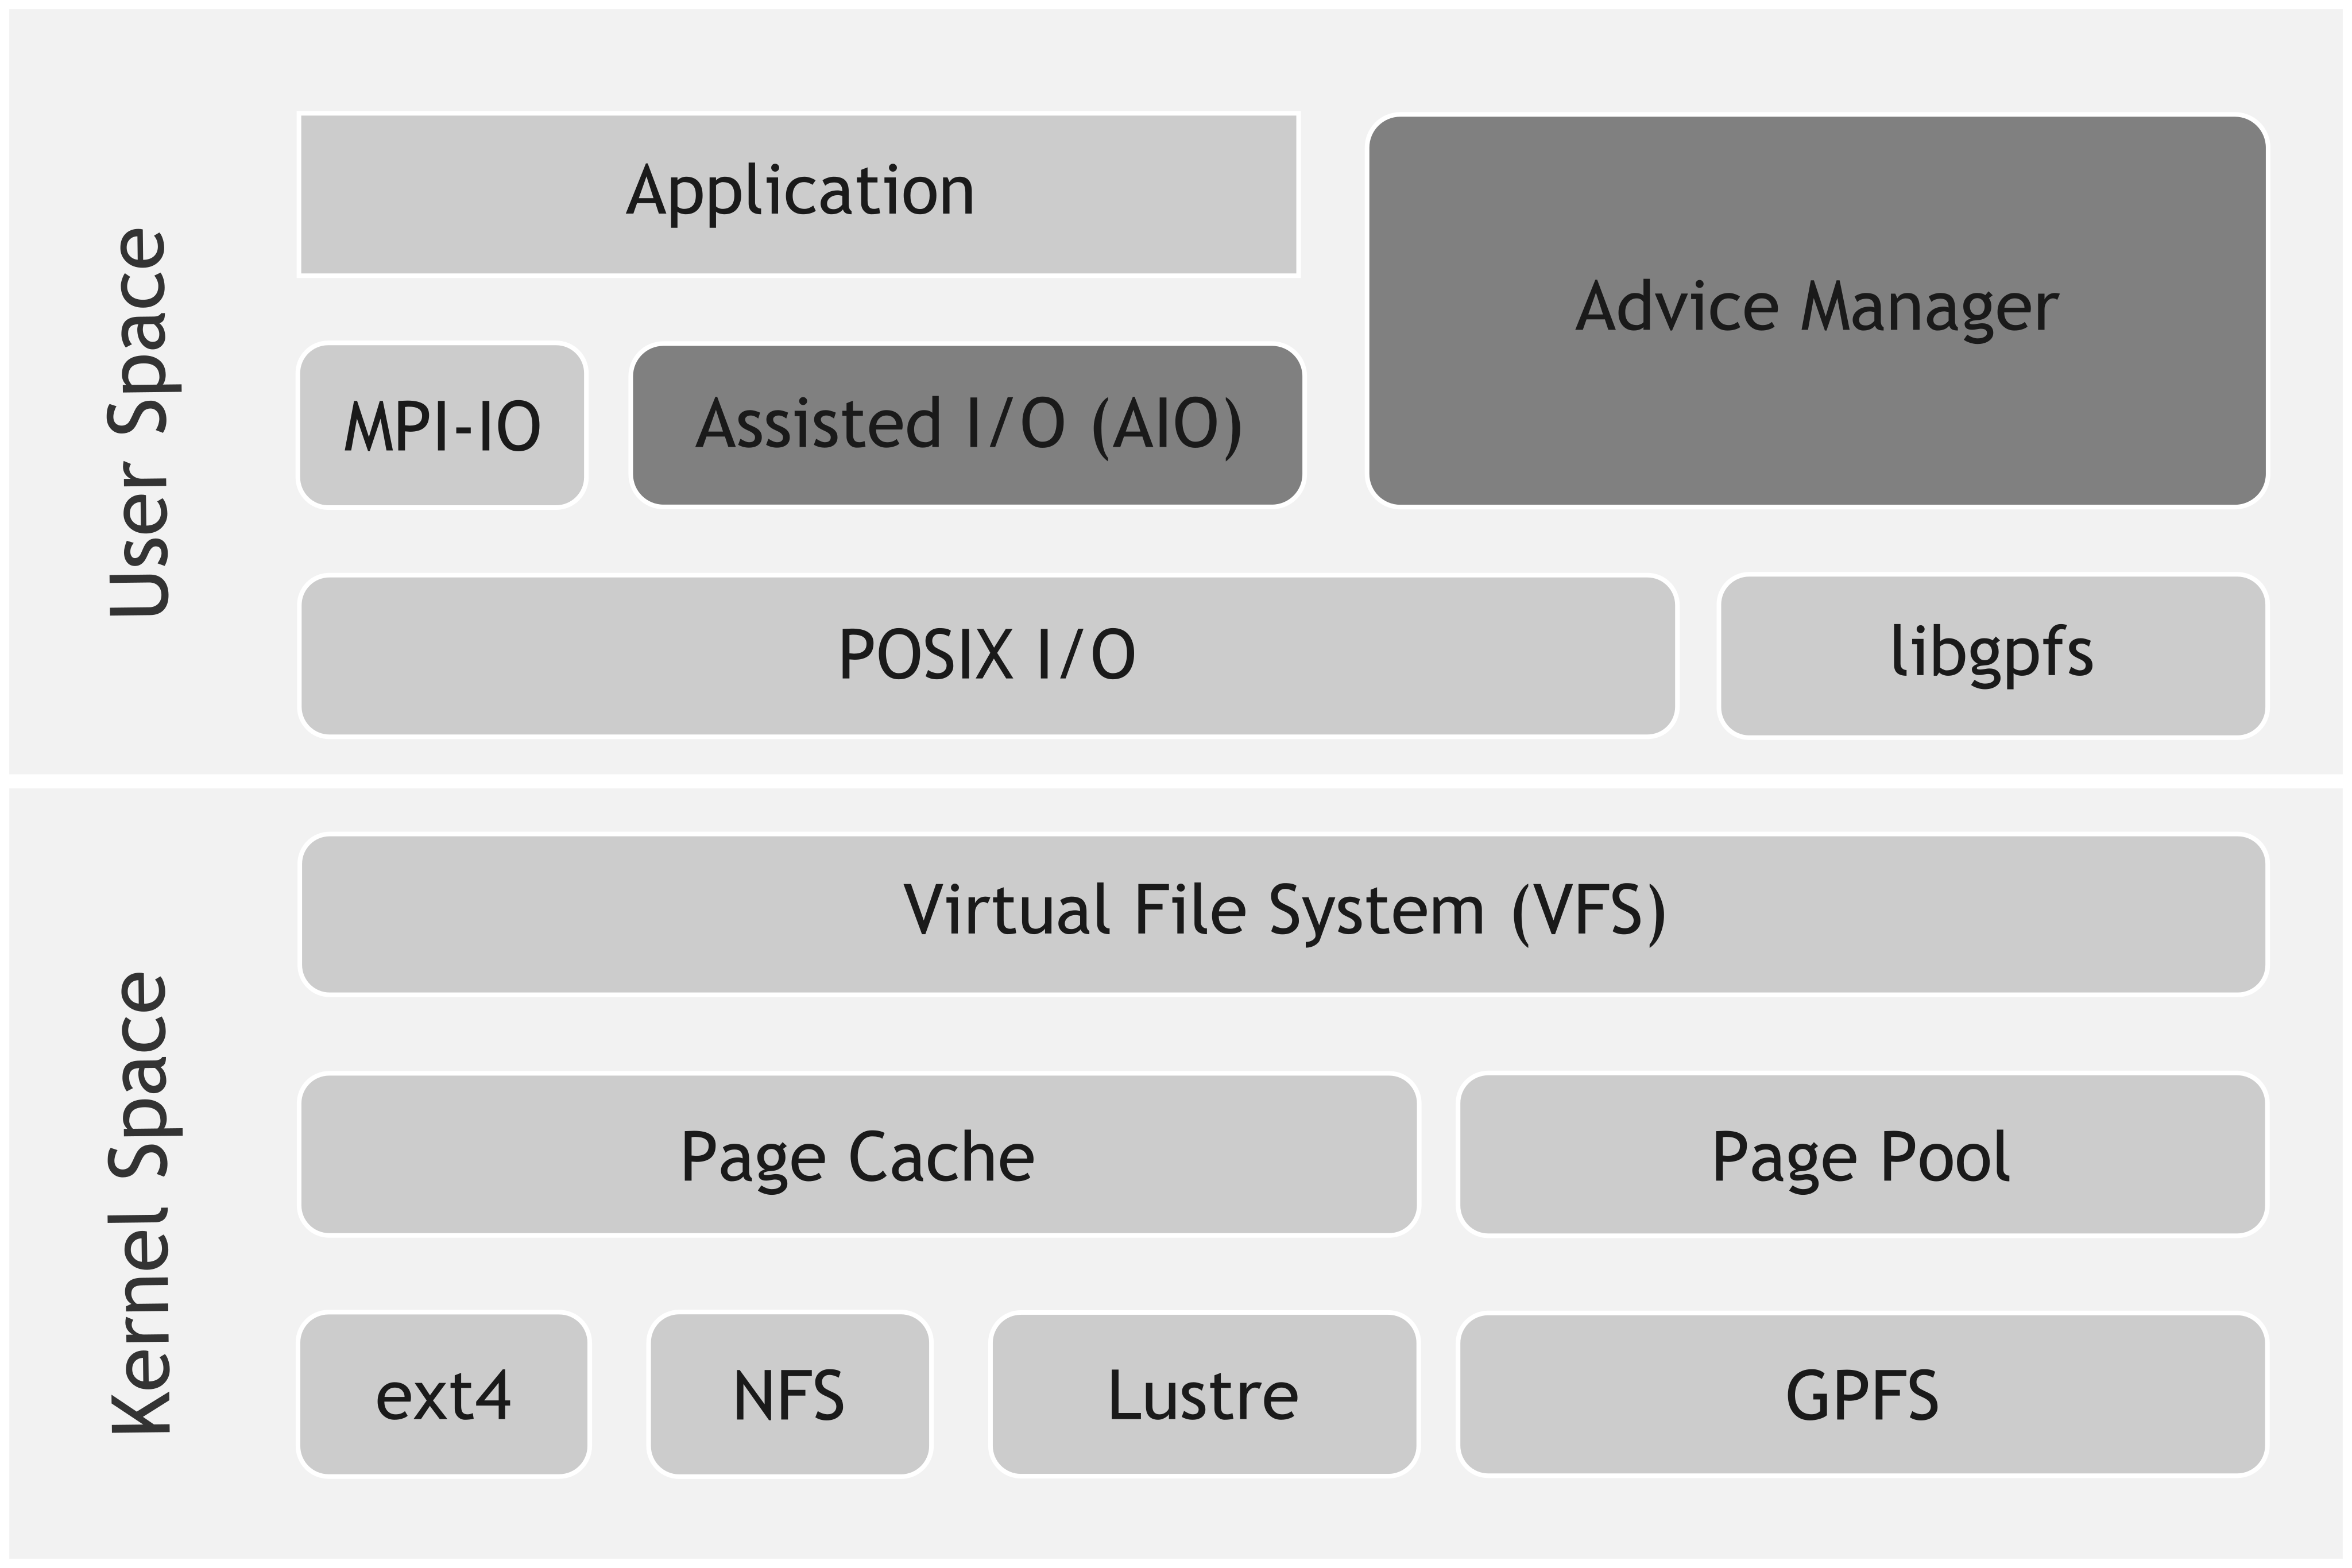
\includegraphics[width=0.8\textwidth]{figures/linux-software-stack-ext}
  \caption{Mercury I/O software stack. \textit{assisted I/O library} and \textit{advice manager} communicate through UNIX domain sockets. The AM binds its socket to the local file system pathname \texttt{/tmp/channel}, while the AIO connects its 
  socket to the same pathname; exactly in the same way they would bind and connect to an IP address if they were located on different nodes in the network. Unix domain sockets are used to pass ancillary data as well as custom messages between the 
  two software entities. Data can reside in a local Linux file system, in Lustre or in GPFS.}
  \label{figure: softwarestack}
\end{figure}

The proposed architecture adds two major contributions. First of all, it allows us to use the Linux advice API as well as the GPFS hints API asynchronously through the \textit{advice manager}. This means that we can effectively overlap I/O and 
computation phases in target applications. Secondly, it enables us to generate POSIX advice and GPFS hints transparently, without the need to modify the application. The information required by the \textit{advice manager} is extracted from 
observations of the application's I/O behaviour~\footnote{How this can be done effectivelly and in a generalized way is itself a research topic and is therefore left as part of future works.} during a set of preliminary runs and then written to 
a configuration file to be used in following runs.

In the rest of this section we describe the different aspects of our design including the interprocess communication between the two software entities and the prefetching request generation using the \texttt{posix\_fadvise()} system call or the 
\texttt{gpfs\_fcntl()} function.

\subsection{Interprocess Communication}
We now describe how interprocess communication is implemented and how messages sent from the \textit{assisted I/O library} are handled by the \textit{advice manager}. Figure~\ref{figure: architecture} depicts the architecture of the two software 
components introduced by our design. The \textit{advice manager} is made up of three smaller modules: a \textit{request manager} (RM) that receives requests sent by the \textit{assisted I/O library}, a \textit{register log} (RL) that keeps track 
of which files are currently handled by the \textit{advice manager}, and an \textit{advisor thread} (AT) that receives read requests from the \textit{request manager} through a queue and issues POSIX advice and GPFS hints.

In order to enable asynchronous prefetching we delegate the task of sending synchronous hints or advice to the \textit{advice manager}. When an application issues an open call for a file, the \textit{assisted I/O library} intercepts it, performs 
the open and then sends a message to the \textit{advice manager}. The message contains a string of the form: \texttt{"\textbf{Register} \textit{pid} \textit{pathname} \textit{fd}"}, plus additional ancillary information explained later. This string 
tells the \textit{request manager} to register the pid of the process opening the file with pathname and file descriptor number, in the register log. As a consequence the \textit{request manager} performs two operations, first it asks the 
\textit{request log} to register the new file. From this point on, future read calls for the file will be monitored by the \textit{advice manager}. Second, it creates a new \textit{advisor thread} that will take care of generating POSIX advice or 
GPFS hints depending on which file system the file resides in. I/O calls coming from the application are never blocked by the \textit{assisted I/O library}. The reason is that the \textit{advice manager} can become congested by too many requests 
coming from different processes and we do not want to reflect this on the behaviour of the application.  %The register operation is described by the flow diagram shown in Figure~\ref{figure: register_operation}.

\begin{figure}[!htb]
  \centering
  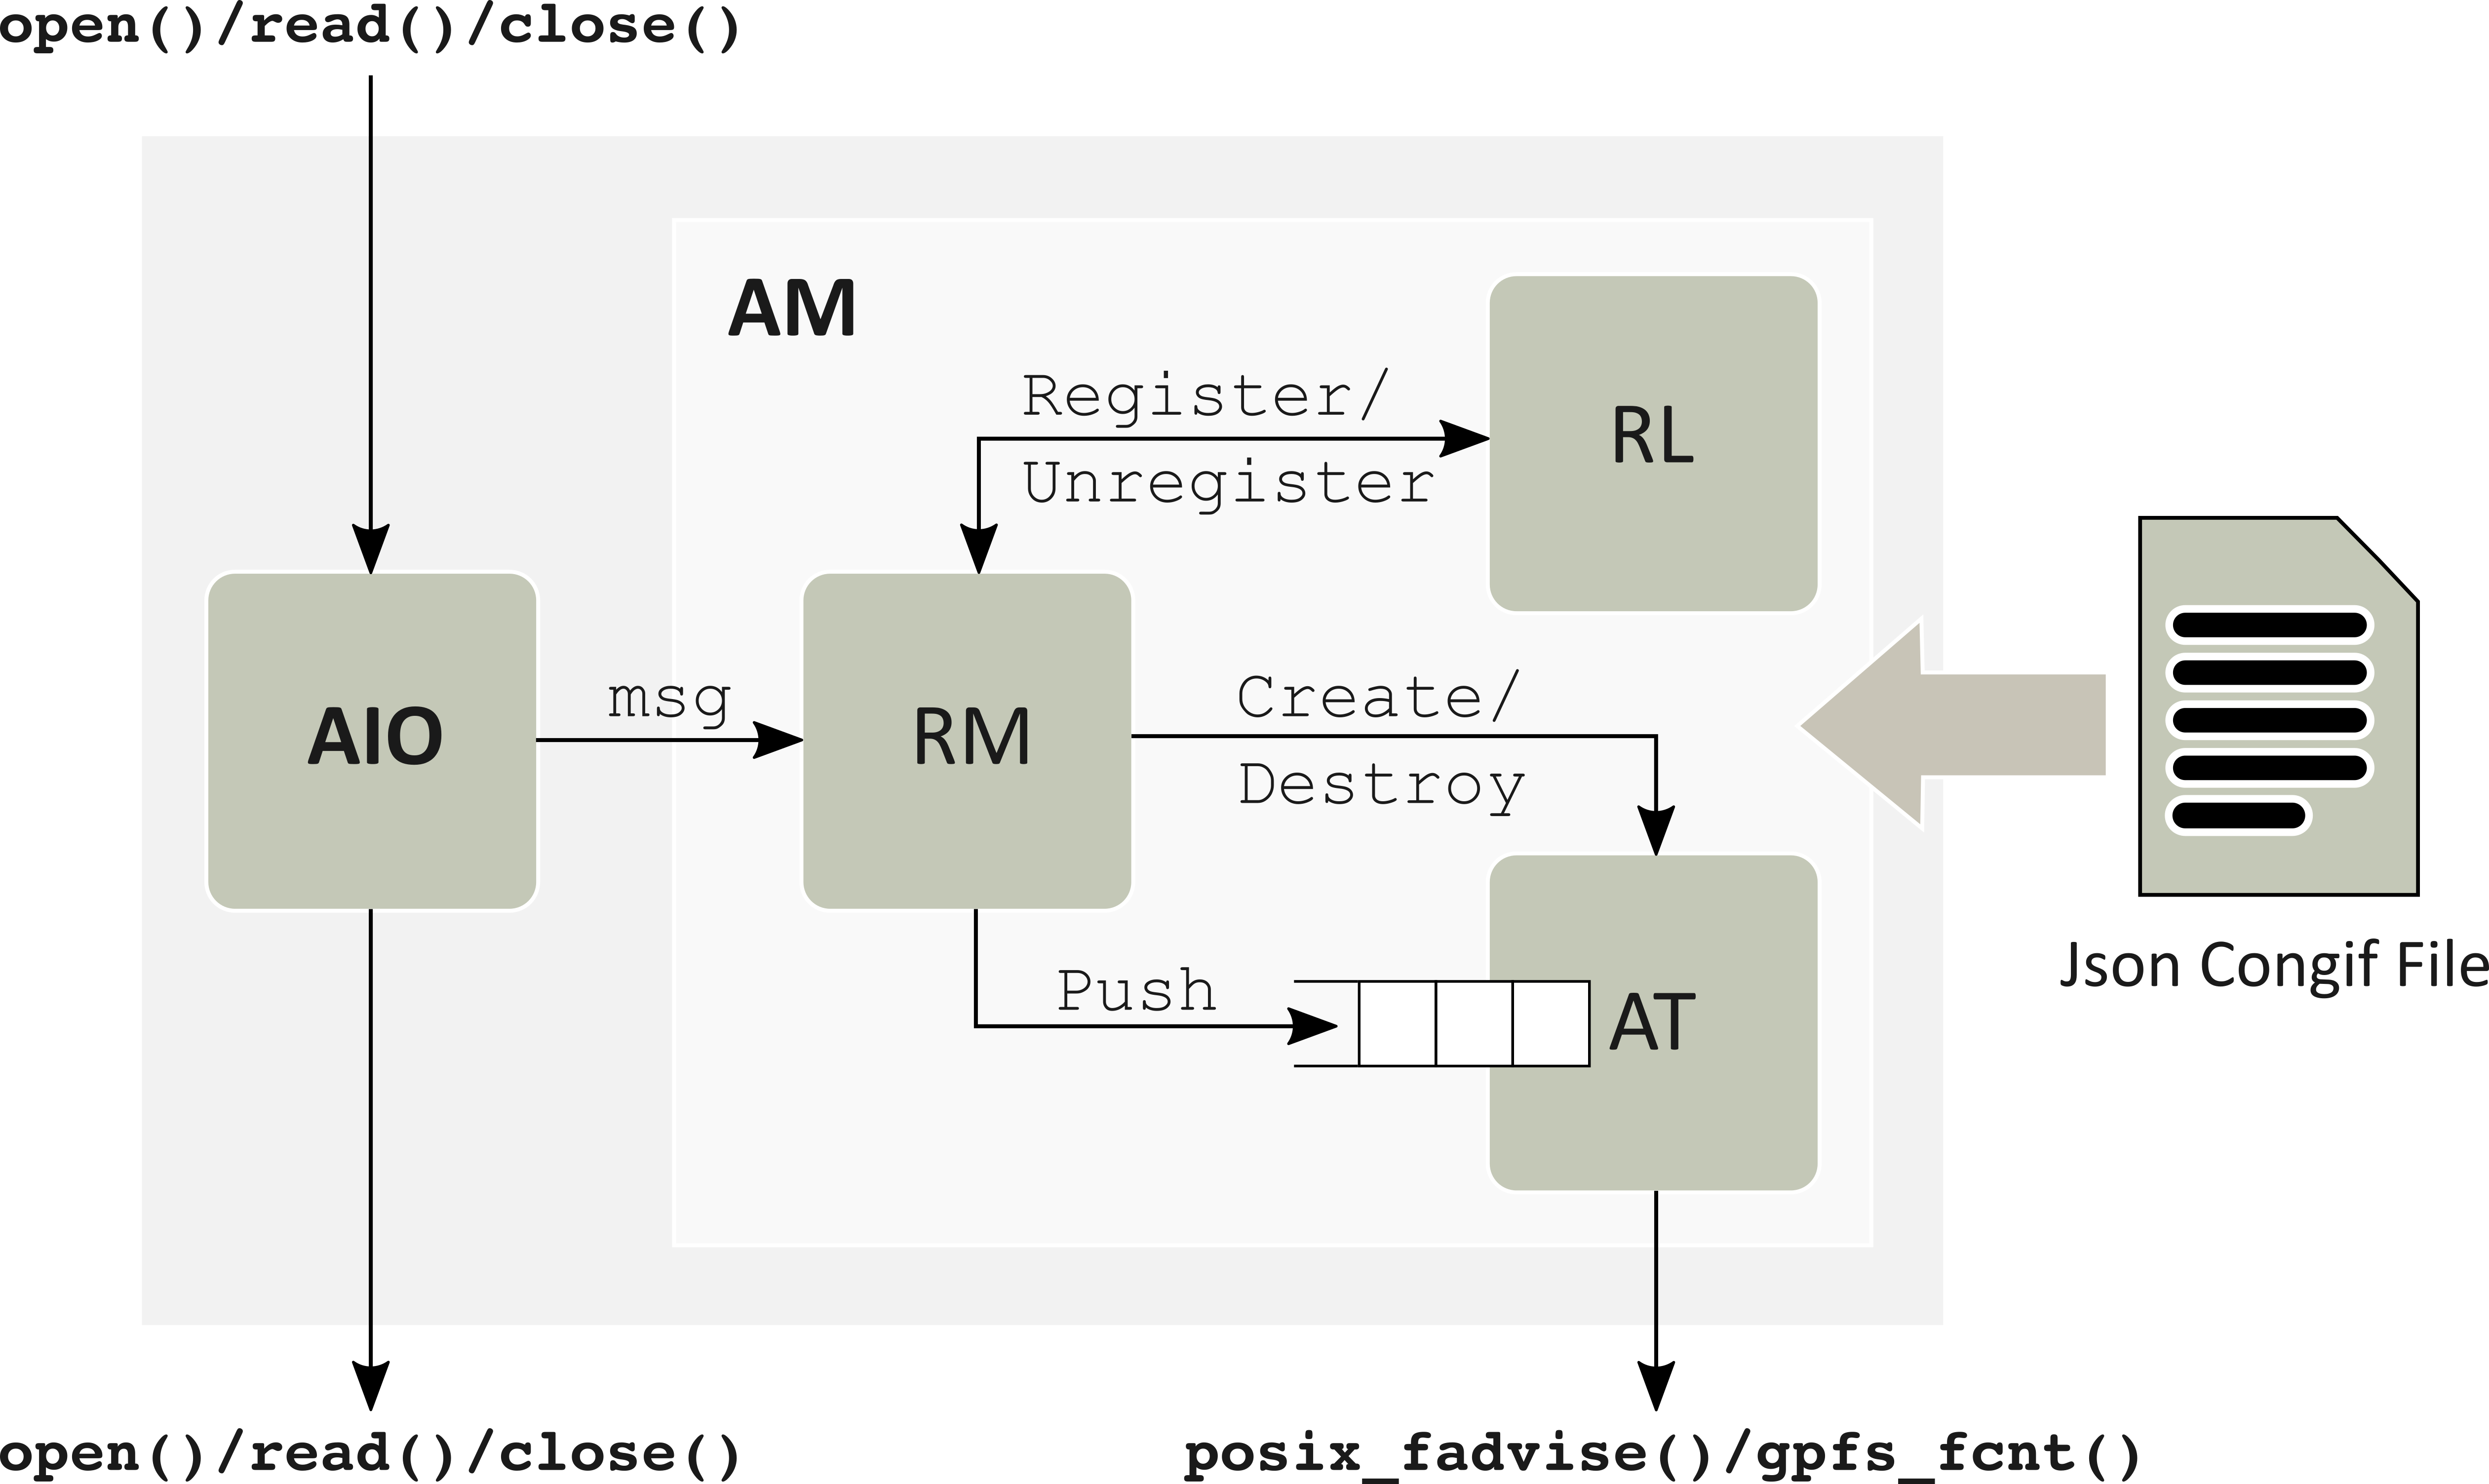
\includegraphics[width=0.8\textwidth]{figures/mercury-architecture}
  \caption{Detailed architecture for the \textit{Advice Manager} (AM) component. This can be further divided into three blocks: \textit{Request Manager} (RM), \textit{Register Log} (RL), and \textit{Advisor Thread} (AT).}
  \label{figure: architecture}
\end{figure}

Both POSIX advice and GPFS hints affect an open file, identified by its file descriptor number. For the \textit{advice manager} to send advice or hints on behalf of the application, it needs to share the open file with the application. When sending 
messages from the \textit{assisted I/O library} to the \textit{advice manager} we use \texttt{sendmsg()}. Besides normal data, this system call allows the transfer of ancillary (or control) information. One use of such information is to send a remote 
process a `file descriptor'~\cite{StevensR13} via a UNIX domain socket~\cite{UnixSock}. These numbers are just an index into the kernel's list of a process's open files. When sending a file descriptor using \texttt{sendmsg()}, the kernel copies a new 
reference to the open file descriptor, and adds it to the receiving process's open files list. The \textit{advice manager} receives a new file descriptor number, (which will likely be different to the number sent), which points to a file descriptor 
shared with the application. This allows us to send hints or advice for the shared file.

\subsection{File Data Prefetching}
POSIX advice and GPFS hints are issued using the \textit{advisor thread} created by the \textit{request manager} during the register operation (Figure~\ref{figure: architecture}). When an application performs a read operation for an open file, the 
\textit{assisted I/O library} sends to the \textit{advice manager} a message containing a string of the form: \texttt{"\textbf{Read} \textit{pid} \textit{fd} \textit{off} \textit{len}"}. This string includes the pid of the process, the application's 
file descriptor number for the file, the offset within the file and the length of the request. The pid and the file descriptor number are used by the \textit{request manager} module only to identify the corresponding \textit{advisor thread}. When the 
correct thread has been identified the \textit{request manager} pushes the offset and the length of the read request into a queue. This queue is accessed by the \textit{advisor thread} that uses the read information to trigger prefetch requests using 
the local file descriptor and keeps track of all the prefetched data using a block cache data structure. %Figure~\ref{figure: read_operation} shows the flow diagram for the read operation. 

The \textit{advisor thread} uses \texttt{posix\_fadvise()} and \texttt{gpfs\_fcntl()} to generate prefetch requests for the underlying file systems (Figure~\ref{figure: architecture}). For files residing in local file systems and Lustre, the 
\texttt{POSIX\_FADV\_WILLNEED} advice from Table~\ref{table: advice_table} is used to bring the data into the kernel page cache. For files residing in GPFS the \texttt{accRangeArray} in the \texttt{gpfsMultipleAccessRange\_t} data structure in 
Listing~\ref{mar} is used to define which blocks of the file should be brought into the GPFS internal cache (page pool). 
The size of the file regions to prefetch is defined inside a Json\footnote{Open standard format that uses human-readable text to transmit data objects consisting of attribute-value pairs (\url{http://www.rfc-editor.org/rfc/rfc7159.txt}).} configuration file, 
loaded at startup by both the \textit{advice manager} and the \textit{assisted I/O library}. This is the only point of configuration for the user and it contains, besides other information, a list of files and directories that the \textit{assisted I/O library} 
should monitor. An example configuration file is shown below. 

\begin{lstlisting}[language=python, caption=Example of Json Configuration File, label={config}]
{
    "File": {
        "Path": "/path/to/target/file",
        "BlockSize": 4194304,
        "CacheSize": 8,
        "ReadAheadSize": 4,
        "WillNeed": {
            "Offset": 0,
            "Length": 0
        }
    },
    "Directory": {
        "Path": "/path/to/target/dir",
        "Random": {
            "Offset": 0,
            "Length": 0
        }
    }
}
\end{lstlisting}

As it can be seen in Listing~\ref{config} the structure of the configuration file is very simple. It allows users to define which files POSIX advice or GPFS hints should be applied to by setting the \texttt{Path} field to the full file path and the regions of 
the file that are likely to be accessed in terms of offset and length. In the case of POSIX advice users can also define directories to which a global advice should be applied (e.g., randomly accessed files in the directory). Additionally, when indicating 
a \texttt{WillNeed} advice users can directly control the caching behaviour of the \textit{advisor thread} block cache. In particular, they can define the granularity of the prefetch request (\texttt{BlockSize}), how many blocks can be fitted into the \textit{advisor thread} 
cache (\texttt{CacheSize}) and how many blocks of data should be read ahead starting from the current accessed block (\texttt{ReadAheadSize}). Clearly the example in Listing~\ref{config} is not exhaustive. More complex configuration files can be generated by administrators 
(or automatic tools) to dynamically change the I/O patterns of applications in order to best adapt them to the underlying storage system.

The replacement policy for the block cache in the \textit{advisor thread} uses an LRU algorithm. In order to prefetch data, the open file is divided into blocks of size `BlockSize' and entire blocks are loaded/released into/from memory as the application 
progresses. In the case of GPFS the \texttt{accRangeArray} hint is used to prefetch up to `ReadAheadSize' blocks ahead starting from the block touched by the current request. When the number of blocks in the cache has reached `CacheSize', if more blocks are 
requested, older blocks will be released using the \texttt{relRangeArray} hint to make space for the new ones. In the case of POSIX advice, the behaviour is the same but blocks are loaded into memory using the \texttt{POSIX\_FADV\_WILLNEED} advice and released 
using the \texttt{POSIX\_FADV\_DONTNEED} advice. The hints interface is automatically selected by the \textit{advice manager} at runtime depending on the file system hosting the target file. 

The \textit{advisor thread} block cache also provides a very basic level of coordination among processes accessing the same file. In fact, different \textit{advisor thread} instances hinting the same file on behalf of different processes share the same block 
cache. Blocks requested by one process will appear in the block cache and future accesses to those blocks by other processes will not trigger new prefetching requests.

In general the configuration file can be used to describe any of the advice listed in Table~\ref{table: advice_table} and the hints listed in Table~\ref{table: hints_table}. To define a new scenario, we may consider a file region accessed sequentially for which 
the \texttt{POSIX\_FADV\_SEQUENTIAL} advice type could be used, and another region accessed randomly for which the \texttt{POSIX\_FADV\_RANDOM} advice type could be used. In this case, the configuration file would contain a list of file regions, specifying which 
type of advice messages are suitable. The right advice will be selected according to which part of the file is being accessed currently. This feature allows us to overcome another limitation of the Linux advice implementation that has been mentioned in 
Section~\ref{section: hints_interface}, namely, the first three advice types apply to the whole file since the implementation in the kernel completely disregards the byte ranges specified by the user.
 
Finally, when the application closes the file the \textit{assisted I/O library} sends to the \textit{advice manager} a message containing a string of the form: \texttt{"\textbf{Unregister} \textit{pid} \textit{fd}"}. This string includes the pid of the process 
and the file descriptor number of the file to be closed. In response to this request the \textit{request manager} tells the \textit{register log} to unregister the file and destroys the \textit{advisor thread}, it also closes its shared copy of the file.

\subsection{POSIX Advice integration with Lustre}
Lustre is a high performance parallel file system for Linux clusters. It works in kernel space and takes advantage of the available page cache infrastructure. Additionally, it extends POSIX read and write operations with distributed locks to provide data 
consistency across the whole cluster. Even though Lustre makes use of the Linux kernel page cache, the previously described POSIX advice syscall has no effect on Lustre. The reason can be understood by looking at Figure~\ref{figure: kernel}. This reports 
the simplified call graph for the Lustre read operation in the file system client. To simplify the explanation, the figure is divided into four quadrants. Along the x-axis we have the native kernel functions (e.g., \texttt{generic\_file\_aio\_read}), separated 
by the Lustre specific functions (e.g., \texttt{lustre\_generic\_file\_read}). Along the y-axis we have page operations (e.g., \texttt{find\_get\_page}) separated by the file operations (e.g., \texttt{generic\_file\_aio\_read}). 

We can notice that Lustre extends the kernel code with additional file and page operations through the Lustre Lite component. These are the functions used by the kernel to fill the file operations table and the address space operations table. The 
\texttt{posix\_fadvise()} system call in the kernel translates into \texttt{fadvise64()}. In the case of \texttt{POSIX\_FADV\_WILLNEED} this function directly invokes \texttt{force\_page\_cache\_readahead()} which has no effect on \texttt{ll\_readpage()}. 
Other advice such as \texttt{POSIX\_FADV\_\{NORMAL,SEQUENTIAL,RANDOM\}} are disabled in Lustre by setting the kernel readahead window size to zero. This is done so that Lustre will not speculatively try to gain a highly-contended lock to fulfil an optimistic 
readahead request.

\begin{figure}[!htb]
  \centering
  \includegraphics[width=\textwidth]{figures/linux_lustre}
  \caption{Simplified function call graph for the read operation in Lustre. For page operations in the Linux kernel the picture also shows the call graph typically followed by local reads as well as the call graph for the 
  \texttt{POSIX\_FADV\_WILLNEED} advice in the \texttt{posix\_fadvise()} implementation (dashed line).}
  \label{figure: kernel}
\end{figure}

In order to enable \texttt{POSIX\_FADV\_WILLNEED} in Lustre we modified the call graph of \texttt{fadvise64()} presented in Figure~\ref{figure: kernel} to invoke the \texttt{aio\_read()} operation in the file operations table for the open file and block 
until all the data has been read into the page cache. In this way we can force the kernel to invoke the corresponding file read operation in Lustre, acquiring locks as appropriate. Of course this mechanism still works with local file systems which eventually 
will end up calling \texttt{force\_page\_cache\_readahead()} as in the original version.

To prevent the new generated read from altering the readahead state of normal read operations, in \texttt{fadvise64()} we create a new \texttt{struct file} using the \texttt{dentry\_open()} routine and set the access mode flag (\texttt{f\_mode}) of the 
new file to \texttt{FMODE\_RANDOM} (which is exactly what the \texttt{POSIX\_FADV\_RANDOM} advice message does to disable readahead for random accessed files). This mechanism works perfectly with local file systems but has no effect on Lustre's readahead 
algorithm which is independent from the Linux kernel readahead. Therefore, \texttt{POSIX\_FADV\_WILLNEED} in the case of Lustre prefetches a bit more data than requested. This is acceptable for now but a future implementation will also modify the Lustre 
code to make sure the behaviour is the same in both cases.

Finally, our kernel patch does not require any user buffer to be provided with the new read operation. To avoid data being copied to user space we pass a null pointer to the \texttt{aio\_read()} routine. Additionally we defined a new \texttt{ki\_flag} 
for the kernel I/O control block (\texttt{kiocb}), that we called \texttt{KIF\_FORCE\_READ\_AHEAD}. This new flag is checked in the \texttt{generic\_file\_aio\_read()} routine and if set the \texttt{do\_generic\_file\_read()} routine is invoked with a 
pointer to the \texttt{file\_read\_actor\_dummy()} routine. \texttt{file\_read\_actor()} is normally the routine responsible for copying the data from the page cache to the user space buffer. Since in our case there is no user space buffer, the dummy 
routine just returns success.

\section{Contributions} \label{section: mercury_related_work}
In the past researchers have tried to alleviate the I/O gap by analyzing I/O patterns and exploiting their knowledge to guide I/O using, for example, data prefetching. Tran and Reed~\cite{TranR04} presented an automatic 
time series modelling and prediction framework for adaptive I/O prefetching, named TsModeler. They combined ARIMA and Markov models to describe temporal and spatial behaviour of I/O patterns at file block level. TsModeler 
was integrated with the experimental file system PPFS2 to predict future accesses and tested against a selected physics code. Several characteristics, such as execution time improvements and cache miss reduction over different 
hardware configurations, are considered in the experiments. The results show that execution time can be reduced by the 30\% in some cases and cache misses can be reduced up to three order of magnitude. 

He et al.~\cite{HeBTAGGMCS13} proposed a pattern detection algorithm, based on the sliding window algorithm in LZ77 as base for building Markov models of I/O patterns at file block level. The model was afterwards used by a FUSE 
based file system to carry out prefetching. Chang and Gibson~\cite{ChangG99}, unlike previous works, did not build mathematical models but instead used speculative execution of the application code to guide data prefetching. Some 
authors have also used code analysis during source code compilation to automatically insert prefetch hints and hide disk latency to applications~\cite{Mowry1996}~\cite{Brown2000}~\cite{Brown2001}.

Other works tried to bring the same idea to higher level I/O libraries such as MPI-IO, HDF5 or PnetCDF to take advantage of the richer semantic, data dependencies and layout information. Chen et al.~\cite{ChenBSTG08} proposed a 
pre-execution based prefetching approach to mask I/O latency. They provided every MPI process with a thread that runs in parallel and takes responsibility for prefetching future required data. Prefetching in the parallel thread 
was enabled via speculative execution of the main process code. Results, with PBench running on top of NFS and PVFS as file systems backend, show execution time reduction and sustained bandwidth improvements. The same authors in
~\cite{Byna2008} proposed to exploit parallel prefetching using a client-side, thread based, collective prefetching cache layer for MPI-IO. The cache layer used I/O pattern information, in the form of I/O signatures, together 
with run-time I/O information to predict future accesses. Experimental results show sustained bandwidth improvements even in this case. 

Chen and Roth~\cite{ChenR10} took inspiration from the collective I/O optimization enabled by ROMIO to design a collective I/O data prefetching mechanism that exploited global I/O knowledge. They compare the sustained bandwidth 
speed-up of individual prefetching with collective prefetching for a parallel benchmarking tool using PVFS2, and demonstrate that the latter performs better than the former by over two fold on average. He et al.~\cite{HEST12} 
proposed to analyze high level data dependencies exposed in PnetCDF, accumulate this knowledge building data dependency graphs and finally use them to perform prefetching.

VanDeBogart, Frost and Kohler have previously used the Linux advice API to build a prefetching library~\cite{VanDeBogartFK09} for programmers to use. Prost et al. integrated the GPFS hint functionalities in the ROMIO ADIO driver 
for GPFS~\cite{ProstTHJK01}. In this context they exploit data type semantic in file views to prefetch parts of the file that will be soon accessed. 

In contrast to previous works, we do the following things differently. We do not try to automatically build mathematical models of I/O patterns and use them to accurately generate prefetching requests nor do we speculatively execute the application 
binary. In fact, we believe that users and administrators have the best understanding about the applications and their systems, and can exploit their knowledge and expertise to improve the storage system performance. We demonstrate that experienced 
users with a deep knowledge of their applications I/O behavior can convert non-optimal I/O patterns, in particular small random reads, into patterns that can be adapted to the underlying file system characteristics, and therefore give optimal 
performance. Furthermore, previously described approaches are not suitable for small random read patterns since they rely on accurate knowledge of I/O behaviour to prefetch every single request one after the other. This still degrades the storage 
system performance due to the large number of I/O requests and seek operations hitting the storage devices. On the other hand, by using the POSIX advice and GPFS hints APIs, we can prefetch the region of the file that will be accessed and filter 
random requests using the cache.

In this work we focus on providing the infrastructure that enables Linux users to access file system specific interfaces for guided I/O without modifying applications and hiding the intrinsic complexity that such interfaces introduce.
